% arara: pdflatex: { shell: yes, synctex: on }
% arara: pdflatex: { shell: yes, synctex: on } if found('log', 'undefined references')

% arara: clean: { extensions: [ aux, log, toc ] }

\documentclass[11pt]{memoir}

\title{Software Security}
\author{Kha Dinh Duy}

\usepackage[utf8]{inputenc}
\usepackage[newfloat]{minted}
\usepackage{csquotes}
\usepackage{caption}
\usepackage{graphicx}
\usepackage[abbreviations]{foreign}
\usepackage{wrapfig}
\usepackage{hyperref} % Hyperlink in refs
\DeclareFloatingEnvironment[fileext=frm,placement={ht},name=listing]{floatcode}
\setlrmarginsandblock{2.5cm}{2.5cm}{*}
\setulmarginsandblock{2.5cm}{2.5cm}{1}
\checkandfixthelayout 


\newenvironment{code}[0]{\begin{floatcode}[tb]}{\end{floatcode}}
% \newenvironment{code}{\captionsetup{type=listing}}{}
% \SetupFloatingEnvironment{listing}{name=Listing, placement={h}}
\usepackage{tikz}

\usepackage[english]{babel}
\usepackage{biblatex}
\addbibresource{references.bib}
% \usepackage[a4paper]{geometry}
% \geometry{
% % left=3.5cm,  
% % right=2.5cm,
% top=2.5cm, bottom=2.5cm,
% headheight=\baselineskip,
% headsep=7mm,
% footskip=7mm
% }


\usepackage[acronym]{glossaries}
\makeglossaries
\newacronym{rop}{ROP}{Return-Oriented Programming}
\newacronym{sfi}{SFI}{Software-based Fault Isolation}
\newacronym{ipc}{IPC}{Inter-Process Communication}
\newacronym{tee}{TEE}{Trusted Execution Environment}
\newacronym{uaf}{UAF}{Use-After-Free}


\usepackage[nameinlink]{cleveref}


\setminted[C]{linenos=true,frame=single,xleftmargin=.8cm}
\setminted[asm]{linenos=true,frame=single,xleftmargin=.8cm}
\begin{document}


\maketitle
\tableofcontents

\makepagenote

\chapter{Core Concepts}
This chapter covers the core concepts that are necessary to understand the following chapters.
Many of the architectural details are omited 

Contents are borrowed from Aaron Bloomfield's Program and Data Presentation course\footnote{\url{http://aaronbloomfield.github.io/pdr/readme.html}} and the textbook \cite{bryant2016computer}

\section{Virtual address space}

\begin{wrapfigure}[18]{r}{.5\textwidth}
    \centering
    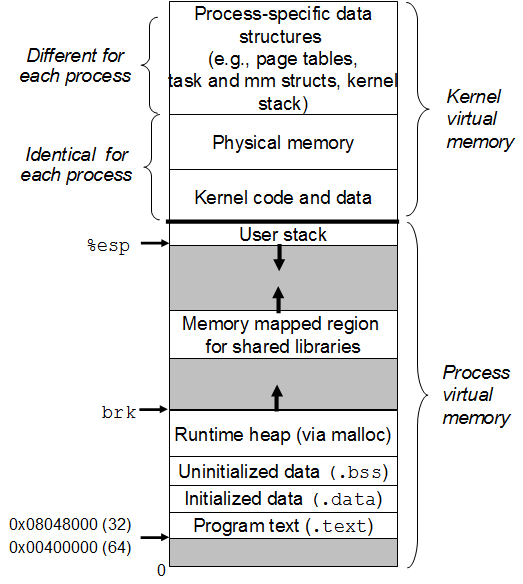
\includegraphics[width=8cm]{figures/malloc1.png}
    \caption{Caption}
    \label{fig:addr_space}
\end{wrapfigure}


\Cref{fig:addr_space}
\section{Stack \& Calling Conventions}
The stack is a first-in, last-out data structure that is used to implement machine-level procedure calls. 
On most architectures, a dedicated register holds the address of the top of the stack, i.e., the \emph{stack pointer}: \texttt{rsp} for x86 and \texttt{sp} for arm64.

Memory on the stack is \emph{allocated} by manipulating the stack pointer.
The stack grows from higher to lower addresses, so allocating memory on the stack requires subtracting the stack pointer value, and deallocating the memory requires adding to the stack pointer. 

On x86, the \texttt{push} instruction 

\subsection{Calling convention}
On each procedure (i.e., function), a \emph{stack frame} is used to store its data, including the local variables, arguments for function calls, and return addresses.
\begin{wrapfigure}[14]{r}{.4\textwidth}
\begin{minted}{C}
int Z(int a, int b, int c){
    return a + b + c;
}
int P(int a, int b){
    int c = 3;
    return Z(a, b, c);
}

int Q(){
    return P(1,2);
}
\end{minted}
\captionof{listing}{My C-Code}
\label{lst:}
\end{wrapfigure}


When procedure \texttt{Q} invokes procedure \texttt{P}, the following actions occur~\cite{bryant2016computer}:
\begin{itemize}
    \item Control transfer: The program counter is set to the address of the \texttt{P}. It is then set to the next instruction after the call inside \texttt{Q} when \texttt{P} returns.
    \item Data transfer: Arguments are passed from \texttt{Q} to \texttt{P}, either on the stack or in registers.
    \item Allocating and deallocating memory: The memory for \texttt{P}'s stack frame is allocated, and then deallocated when \texttt{P} returns.
\end{itemize}
In x86, the \texttt{call} instruction push the return address onto the stack, then change the instruction pointer to the address of the target function.

the \texttt{ret} instruction pop the return address on the stack into the program counter.

A procedure usually consists of three components: the \emph{prologue}, the \emph{function body} and the \emph{epilogue}.
\begin{itemize}
    \item The \emph{prologue} performs the necessary setup steps, which include saving the return address onto the stack and allocating the stack frame.
    \item The function \emph{body} contains the actual implementation of the procedure.
    \item The \emph{epilogue} deallocates the stack frame and transfers the control back to the previous function.
\end{itemize}


\begin{figure}[ht]
\begin{minted}{asm}
Z(int, int, int):
    // Prologue
    mov DWORD PTR [rsp-4], edi  // store a into stack
    mov DWORD PTR [rsp-8], esi  // store b into stack 
    mov DWORD PTR [rsp-12], edx // store c into stack
    // Function body
    ...
    // Epilouge
    ret
P(int, int):
    // Prologue
    sub rsp, 24                 // Allocate 24 bytes on stack
    mov DWORD PTR [rsp+4], edi  // store a into stack   
    mov DWORD PTR [rsp], esi    // store b into stack 
    mov DWORD PTR [rsp+20], 3   // store c = 3 into stack
    // Function body
    mov edx, DWORD PTR [rsp+20]
    mov ecx, DWORD PTR [rsp]
    mov eax, DWORD PTR [rsp+4]
    mov esi, ecx
    mov edi, eax
    call    Z(int, int, int)    
    // Epilogue
    add rsp, 24                 // Deallocate 24 bytes
    ret
Q():
    // Prologue
    mov esi, 2          // prepare 2nd argument in esi 
    mov edi, 1          // prepare 1st argument in edi 
    call P(int, int)
    // Epilogue
    ret
\end{minted}
\captionof{listing}{My C-Code}
\end{figure}

The same code is compiled to the following on armv8:
\begin{code}
\begin{minted}{asm}
Z(int, int, int):
    // Prologue
    sub sp, sp, #16     // allocate 16 bytes on stack
    str w0, [sp, 12]
    str w1, [sp, 8]
    str w2, [sp, 4]
    // Function  body
    // ...
    // Epilogue
    add sp, sp, 16
    ret
P(int, int):
    // Prologue
    str x30, [sp, -48]! // allocate 48 bytes on stack 
                        // + store return address
    str w0, [sp, 28]    // store a into stack
    str w1, [sp, 24]    // store b into stack
    mov w0, 3           // store c = 3 into w0
    // Function body
    str w0, [sp, 44]    // move c from w0
    ldr w2, [sp, 44]    // into w2
    ldr w1, [sp, 24]    // prepare 2nd argument
    ldr w0, [sp, 28]    // prepare 1st argument
    bl  Z(int, int, int)
    ldr x30, [sp], 48   // deallocate 48 bytes 
                        // + load return address
    ret
Q():
    str x30, [sp, -16]!
    mov w1, 2
    mov w0, 1
    bl P(int, int)
    ldr x30, [sp], 16
    ret
\end{minted}
\label{lst:example-arm}
\captionof{listing}{Code}
\end{code}
% \begin{itemize}
%     \item the arguments are passed on the stack
%     \item the return address is pushed onto the stack
% \end{itemize}

ARM uses a LR register to store the return address. 
The \texttt{bl} instruction saves the return address into the LR register (\texttt{x30}), then update the program counter to the target function's address.
ARM's \texttt{ret} instruction updates PC to the address inside \texttt{x30}.

When the called function is not a leaf function, return address need to be spilled into the stack so that it can be used for other call.

In the example, at lines 9 and 11, the return address is stored into the stack, and then restored.
The load instruction on line 9 uses arm's \emph{pre-indexing mode}\footnote{https://developer.arm.com/documentation/102374/0100/Loads-and-stores---addressing} (indicated by the \texttt{!} symbol).
It first add the offset, \texttt{-16} to \texttt{sp}, then store \texttt{x30} into the memory indexed by the new \texttt{sp}.
Functionally, this is equivalent to x86's \texttt{push} instruction.


 
\section{Heap}
The heap is the storage for \emph{dynamically} allocated memory.
This means that heap memory must be obtained explicitly with an allocator.

Unlike the stack where memory allocations are automatically done by the compiler (i.e., each allocation has a corresponding de-allocation), the responsibility of managing the heap is up to the programmer.


% Those bugs are further discuss



\chapter{Attacker's Point of View}
\section{Attacker goals}
\begin{itemize}
    \item Denial of service
    \item Arbitrary code execution
    \item Stealing information
    \item Create an entry point for other attacks
\end{itemize}

\section{Memory corruption}
% Low-level vs. high-levvel exploits
In this article, we only concern with \emph{low-level exploits}. 
We assume that the program logic is implemented perfectly, i.e., no logic bugs.


Memory corruption is the root of all low-level exploits.
This means that a memory-safe program is unexploitable.

%Why are there corruption?
Memory corruption happens because of the memory unsafe nature of low-level programming languages (\ie, C/C++).



\section{Attack primitives}
\subsection{Control-flow hijacking}
An attacker performs control-flow hijacking by altering the victim program's \emph{control flow} (i.e., the program's program counter) into their intended location. 
A control flow graph is a graph where

\subsection{Forward edges \& backward edges}

Forward edge control flow transfers

\subsection{Return-oriented programming (ROP)}
\gls{rop} is a backward edge hijaking attack that corrupts the return address saved on the stack to the attacker's address.
In practice, ROP is

\section{Type confusion}

\chapter{Defenses}



\section{Sanitizers}
\subsection{Sanitizer vs. Exploit Mitigation}
Sanitizers can pinpoint the exact location where memory a memory error occur, while exploiting mitigation techniques only detect/prevent exploit attempts.

Sanitizer is often employed before the deployment of the program (\ie, offline) for testing.
Hence, they can have a high overhead.
On the other hand, exploit mitigation is deployed at production.  
A mitigation technique that has a high overhead often never sees adoption.

False positive detections are unacceptable in exploit mitigation, because it terminate the proram. 
On the other hand, false positive in sanitizer is acceptable since the developer can review the bug report.




\section{Exploit Mitigations}
Guaranteeing full memory safety is often infeasible due to .
\subsection{Control-flow integrity}

\subsection{Code pointer integrity}
\cite{szekeres2013sok}


\section{Fuzzing}

\section{Safe Languages}

\section{Isolation/Sandboxing/Compartmentalization}
One of the earliest ideas in protecting computer systems is to divide the programs into multiple \emph{protection domains}, each with different capabilities based on their trustworthiness~\cite{lampson1974protection}.
Following this idea, another approach to exploit prevention is to \emph{sandbox} untrusted/error-prone components such that vulnerabilities in those components do not affect other components.


The process model of OSes is one the prime example of sandboxing.

We refer to the process of subdividing an existing program into smaller components as \emph{compartmentalization}.

Compartmentalization provides several benefits.
\begin{itemize}
    \item Smaller attack surface
    \item Smaller protection area
\end{itemize}


\subsection{Determining Isolation Boundary}
There are cases where the isolation boundary is clearly separated.
The first case is libraries and packages; the developers of those software commonly  the least expose a well-defined set of APIs.
For packages, there are dependencies to other packages.

The second case is software with extensible modules, where the kernel is a prime example.
Linux kernel allows loading of kernel modules. 
It is natural to isolate those modules.
Hhwever, it is challenging due to ...


On the hand, retrofitting isolation into existing software that is not written with compartmentalization in mind often requires significant engineering efforts.
There are many research works that aid the process of program splitting through automatic program boundary identification and generation of cross-boundary communication~\cite{huang2022ksplit,kilpatrick2003privman,bittauwedge,liu2017ptrsplit,gudka2015clean,lind2017glamdring,almakhdhub2020mu}.


Performing compartmentalization on complex software such as the kernel is especially challenging.



\subsection{Isolation primitives}
\subsubsection{Process isolation}

\subsubsection{In-process isolation with hardware primitive}

\subsubsection{Software-based Fault Isolation (SFI)}

\paragraph{Sandboxing Compiler}
Sandboxing compiler 

\paragraph{Sandboxing Verifier}
Native client.

\subsection{Limitations}
Isolation is not the perfect solution.

The interface between the sandbox and the trusted part needs to be carefully written to avoid vulnerabilities.



Consider the case where an untrusted processing library is sandboxed.

For process-level isolation, data need to be copied between process through \gls{ipc} channels, which introduce significant overhead.

For this reason, it is common to use in-process isolation primitives such as \gls{sfi} to isolate the memory accesses of the untrusted libraries.

To avoid copying, a natural solution is to use a shared memory region accessible by both the host and the untrusted library.

However, this leads to additional attack vectors.


\chapter*{Further reading}

\newcommand{\furthercite}[1]{\textbf{\citeauthor{#1}. \citetitle*{#1}~\cite{#1}}}
\begin{itemize}
    \item \furthercite{erlingsson2010lowlevel}: examples of low-level vulnerabilities.
    \item \furthercite{szekeres2013sok} and \furthercite{song2019sok}: Excellent summarization of the challenges in memory safety, the mitigation approaches, and the current state-of-the-art in mitigation. 
    
\end{itemize}


% \bibliographystyle{IEEEtran}
% \bibliography{IEEEabrv,references}
\printglossaries

\printbibliography

\end{document}
